\documentclass[paper=a4,10pt]{scrartcl}

\usepackage[utf8x]{inputenc}
\usepackage[ngerman]{babel}
\usepackage[T1]{fontenc}

\usepackage{graphicx}
\usepackage{float}
\usepackage{subcaption}

\usepackage{fancyref}

\usepackage[numbers,square,sort]{natbib} %praktikumsquellenvorgabe
\usepackage{amsmath}
\usepackage{amssymb}

\usepackage{url}
\usepackage{hyperref}

\usepackage[a4paper, includehead, includefoot]{geometry}
\geometry{left=2cm, right=2cm, top=2cm, bottom=2cm}

\begin{document}

\title{Ma-Notizen}
%\author{Author's Name}

\section{Matching}
\subsection{Definition}
Sei $G=(V,E)$ ein endlicher, ungerichteter Graph. Eine Menge $M\subseteq E$ ist ein Matching, wenn es keine zwei Kanten in $M$ gibt, welche inzident zum selben Knoten sind, also den selben Knoten enthalten.

\paragraph{maximal matching}
Ein Matching $M$ heißt maximal matching (nicht erweiterbar), wenn es keine weitere Kante $e \in E \setminus M$ gibt für welche $\{ e\} \cup M$ eine weiteres gültiges Matching wäre.

\paragraph{maximum matching}
$M$ heißt maximum matching (größtmögliches Matching), falls $M$ von allen möglichen Matchings die größte Kardinalität aufweist. Maximum matchings sind auch maximale Matchings und die Mächtigkeit eines Maximum matchings wird Matchingzahl genannt und als $\nu(G)$ notiert.

\paragraph{perfekte matchings}
$M$ ist perfekt, wenn $2 \cdot |M| = V$ gilt, also jeder Knoten des Grapheneinmal in den Kanten in $M$ vorkommen. Perfekte Matchings sind maximum matchings und damit auch maximal. 

\subsection{Eigenschaften}
Seien $A$ und $B$ zwei maximale matchings. 

\begin{itemize}
\item Jede Kante in $B \setminus A$ kann höchstens mit zwei Kanten in $A \setminus B$ benachbart sein (Kanten nennt man benachbart, wenn sie einen Knoten teilen). \\
\textit{Eine Kante, die in $B \setminus A$, also in $B$, aber nicht in $A$ vorkommt hat nur zwei Knoten und da $A$ ein Matching ist, kann es in $A$ nur maximal zwei Kanten geben, die inzident zu diesen Knoten sind (entweder zwei Kanten von denen jeweils eine inzident zu eine der beiden Knoten ist, oder nur einer der Knoten ist von $A$ abgedeckt). Da es also nur maximal zwei Kanten in $A$ geben kann, welche mit einer Kante in $B \setminus A$ benachbart sein können, gilt dies auch für $A \setminus B$ (die Menge wird dadurch ja nur kleiner, aber das gilt schon für die Große).}

\item Jede Kante in $A \setminus B$ grenzt an (mindestens?) eine Kante in $B \setminus A$, weil $B$ nicht erweiterbar ist.\\
\textit{Eine Kante, die in $A \setminus B$ vorkommt, hat wieder zwei Knoten $v, w$. Es kann nicht sein, dass keiner von den beiden Knoten in einer Kante in $B$ vorkommt, weil sonst könnte man $B$ um die Kante $\{v, w\}$ erweitern, was aber per Definition nicht möglich ist. Also werden entweder beide oder nur einer in Kanten von $B$ berücksichtigt. So oder so ist mindestens ein Knoten in einer Kante in $B$ drin und damit benachbart zur Anfangskante aus $A \setminus B$. Jetzt noch die Frage, warum in $B\setminus A$: Die Kanten, die jetzt $v$, $w$ oder beide berücksichtigen können gar nicht Teil von $A$ sein, da ja jeder Knoten nur einmal im Matching auftauchen darf.}
\end{itemize}

Es gilt also: 
\begin{align}
|A\setminus B| \le 2 \cdot |B\setminus A|
\end{align}
$|B \setminus A|$ darf höchstens halb so klein sein, wie $|A \setminus B|$.\\
\textit{In wie fern liefern die Aussagen Hinweise zu den Größen der Mengen? Nach der zweiten Aussage gibt es zu jeder Kante in $A \setminus B$ mindestens eine Nachbarkante in $B\setminus A$, jedoch können da Kanten auch mehrfach als angrenzende Kanten benutzt werden. Jedoch nach der ersten Aussage jede maximal doppelt.\\
Wenn das Gleichzeichen gilt, wird jeder Kante in $A\setminus B$ eine Kante in $B\setminus A$ zugeordnet, die noch zu genau einer anderen Kante benachbart ist. Da jede Kante benachbart mit mindestens einer ist, $B \setminus A$ aber mindestens halb so groß sein muss, damit alle benachbart mit einer Kante aus der zweiten Menge sein können, ist das der worst case und ansonsten ist $B \setminus A$ mehr als halb so groß. Wenn $B\setminus A$ kleiner als halb so groß wie die linke Menge wäre, könnte nicht mehr jeder Kante eine andere als Nachbar zugeordnet werden, da jeder eine zugeordnet werden muss, aber für jeweils höchstens zwei Kanten nur ein Nachbar gemeinsam sein darf.}\\\\
Jetzt da das geklärt ist, kann man schnell schreiben:
\begin{align*}
|A| = |(A \cap B) \cup (A\setminus B)| = |A \cap B| + |A\setminus B| \le 2\cdot |A \cap B| + 2 \cdot |B\setminus A| = 2 \cdot |(A \cap B) \cup (B \setminus A)| = 2\cdot |B|,
\end{align*}
also
\begin{align}
|A| \le 2 \cdot |B|
\end{align}
und da die Bezeichnungen $A$ und $B$ von Anfang an willkürlich gewählt waren, gilt das genauso auch anders herum.



%\textit{Jede Kante in $A \setminus B$ grenzt nach meinem Verständnis an mind. eine Kante in $B\setminus A$. Das bedeutet, dass die Menge $B \setminus A$ mindestens genauso groß sein muss, wie $A\setminus B$, also $|A\setminus B| \le |B\setminus A|$ }

%\textit{Aus der ersten Aussage würde ich ableiten, dass $|B\setminus A| \le 2 \cdot |A\setminus B|$. Da kann man dann auch einfach die Buchstaben vertauschen, aber wozu brauche ich die zweite Aussage?}

\section{Knotenüberdeckungsproblem}
Dieses Problem fragt danach, ob es zu einem geg. einfachen Graphen $G$ und einer Zahl $k$ ein Vertexcover von $G$ der Größe höchstens $k$ gibt. Also ob es eine $k$-elementige Teilmenge $K \subset V$ gibt, sodass jede Kante des Graphen inzident zu mindestens einem Knoten $v \in K$ ist.

\section{Bipartiter Graph}
Ein einfacher Graph $G=(V,E)$ heißt bipartit, falls sich seine Knoten in zwei disjunkte Teilmengen $U$ und $W$ aufteilen lassen, sodass zwischen den Knoten innerhalb beider Teilmengen keine Kanten verlaufen. Die Mengen $U$ und $W$ bezeichnet man dann als Partitionsklassen (englisch parts). Man schreibt dann oft $G = (U, V, E)$ um einen bipartiten Graphen zu beschreiben, dessen Partition die parts $U$ und $V$ hat.
Ein Graph heißt vollständig bipartit, falls eine Bipartion $\{ U, V\}$ existiert, sodass jeder Knoten aus $U$ mit jedem Knoten in $V$ verbunden ist.

\subsection{Matching}
Beim Matching bei bipartiten Graphen geht es darum, Kanten zwischen den parts zu matchen. \textit{Es geht ja auch nur so, da es zwischen Knoten eines parts ja gar keine Kanten gibt.}

\begin{itemize}
\item Die Größe einer minimalen Knotenüberdeckung und eines maximum Matching stimmen auf bipartiten Graphen überein. \textit{Noch keine Gedanken zu gemacht.}


\end{itemize}

\section{Factor-Graph}
Ein Factor-Graph ist ein bipartiter Graph der die Faktorisierung einer Funktion darstellt. Sei eine Faktorisierung der Funktion $g(X_1, X_2, \dots X_n)$ gegeben:
\begin{align}
g(X_1, X_2, \dots X_n) = \prod_{j=1}^m f_j(S_j)
\end{align}
mit $S_j \subseteq \{X_1,X_2, \dots, X_n\}$
\textit{Das heißt, dass sich die Funktion $g$ darstellen lässt als Produkt von $m$ Funktionen von Teilmengen der ursprünglichen Parametermenge. Beispielsweise eine Funktion $g(X_1, X_2, X_3) = f_1(X_1)f_2(X_1, X_2)f_3(X_1, X_2)f_4(X_2, X_3)$.}\\
Der zu einer Faktorisierung gehörende Factor-Graph $G(X,F,E)$ besteht aus Variablenknoten $X=\{X_1, X_2, \dots, X_n\}$, Factor vertices $F=\{f_1, f_2, \dots, f_m\}$ und wie ein normaler Graph gibt es noch die Kanten $E$, wobei die Kanten in Abhängigkeit der Faktorisierung vorliegen: Es existiert eine ungerichtete Kante zwischen einem Variablenknoten $X_k$ und dem factor Knoten $f_j$genau dann, wenn (iff) $X_k \in S_j$. Es wird dabei laut Wiki angenommen, dass die Funktion $g(X_1, \dots, X_n) \in \mathbb{R}$ gilt.

\subsection{Beispiel}
Angenommen wir haben wieder die Beispielfaktorisierung $g(X_1, X_2, X_3) = f_1(X_1)f_2(X_1, X_2)f_3(X_1, X_2)f_4(X_2, X_3)$, dann ist dazu in Abb. \ref{fig:factorgraph} ein korrespondierender Factor-Graph dargestellt. 

\begin{figure}[H]
\centering
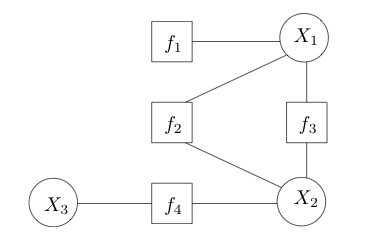
\includegraphics[scale=1]{../bilder/Factorgraph.jpg}
\caption{Beispielfactorgraph}
\label{fig:factorgraph}
\end{figure}
Jede Factornode ist mit den zugehörigen Variablenodes verbunden. Man kann noch erkennen, dass es im Graphen einen Zyklus gibt. Das liegt daran, dass sowohl $f_2$, also auch $f_3$ die Argumente $X_1, X_2$ haben. Da sich beide Faktoren sozusagen aus den selben Argumenten zusammensetzen lassen, kann man diese beiden Faktoren auch zu einem zusammenfassen und der Graph wird zu einem Baum. Das ist relevant, da message passing algorithmen exakt auf Trees funktionieren, während sie für Graphen mit Zyklen nur Approximationen liefern. 

\subsection{Graphen zu Faktorgraphen}
In einem Bsp-paper wird zu einem normalen ungerichteten Graphen ein Factorgraph assoziiert, indem für jeden Knoten ein factor-Knoten gesetzt wird und in jede Kante ein Variableknoten, welcher dann mit zwei Kanten zwischen den factor-Knoten wieder verbunden wird. 

\end{document}